\begin{frame}
    \frametitle{Filtro de Partículas (Particle Filter)}
    \note{Información extraída de Vídeo de Cyrill Stachniss https://youtu.be/MsYlueVDLI0}
    \footnotesize
    \begin{itemize}
        \item Con EKF estamos restringidos a distribuciones Gaussianas.
        \item Cuando usamos EKF obtenemos una Distibuión Gaussiana que describe dónde se encuentra el robot.
        \item En Particle Filter utilizamos partículas o hipótesis que describen dónde podría estar el robot.
        \item En vez de tener una forma paramétrica como es EKF, que describimos la distribución de probabilidad con los parámetros media $\mu$ y covarianza $\covariance$. Partible Filter utiliza muestras no-paramétricas como hipótesis sobre dónde el robot podría estar.
    \end{itemize}
    
    
   	\begin{center}
        \movie[loop]{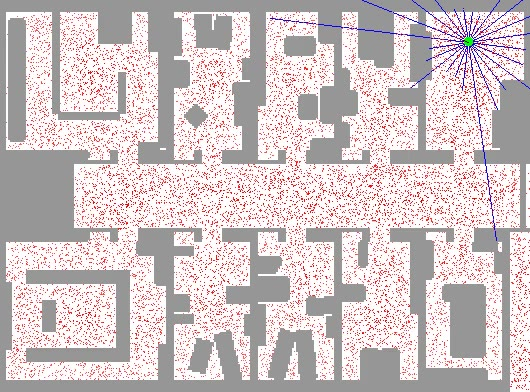
\includegraphics[width=0.4\columnwidth]{images/particle_filter/particle_filter_video.jpg}}{videos/particle_filter.mp4}
    \end{center}
    
    \note{Vídeo extraído de https://rse-lab.cs.washington.edu/projects/mcl/animations/global-floor.gif}
    
\end{frame}

\begin{frame}
    \frametitle{Aproximación de una Función}
    \note{Información extraída de Vídeo de Cyrill Stachniss https://youtu.be/MsYlueVDLI0}
    \footnotesize
    
    \begin{itemize}
        \item Objetivo: Poder estimar cualquier \textbf{distribución de probabilidad arbitraria}.
    \end{itemize}
    
    \begin{center}
    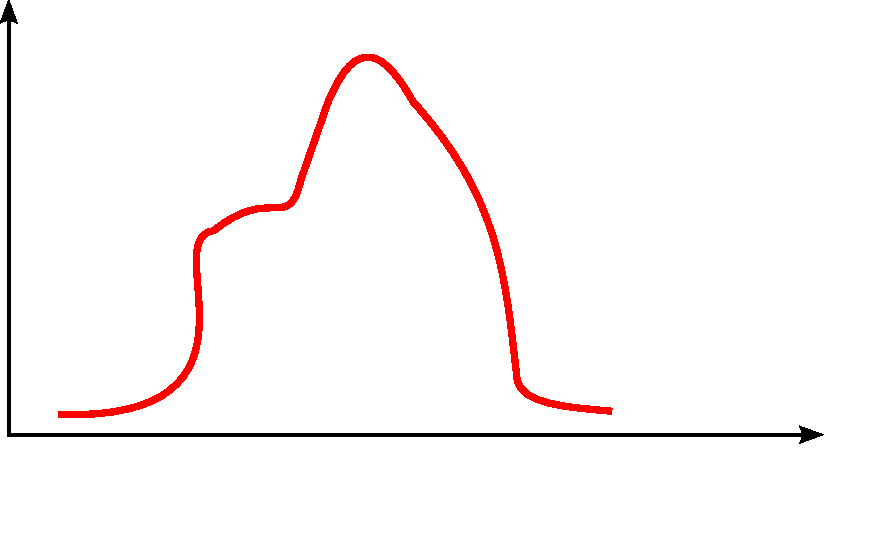
\includegraphics[width=0.5\columnwidth]{./images/particle_filter/arbitrary_distribution.pdf}
    \end{center}
    
\end{frame}

\begin{frame}
    \frametitle{Utilizando Muestras (Partículas)}
    \note{Información extraída de Vídeo de Cyrill Stachniss https://youtu.be/MsYlueVDLI0}
    \footnotesize
    \begin{itemize}
        \item \textbf{Múltiples muestras} para representar una distribución de probabilidad arbitraría
        \item Las muestras son están más agrupadas en algunas áreas en otras menos. La cantidad de partículas por unidad de área describe que tan probable es que el robot se encuentre en esa área.
        \item Cada muestra está acumulando un poco de ``masa de probabilidad''.
        \item Las muestra puede ser vista como una aproximación a la función de densidad de probabilidad (pdf).
        \item Para obtener la pdf, hay que integrar sobre una cierta área de manera de obtener la probabilidad matemática de que el robot se encuentre en dicha área.
    \end{itemize}
    
    \begin{center}
    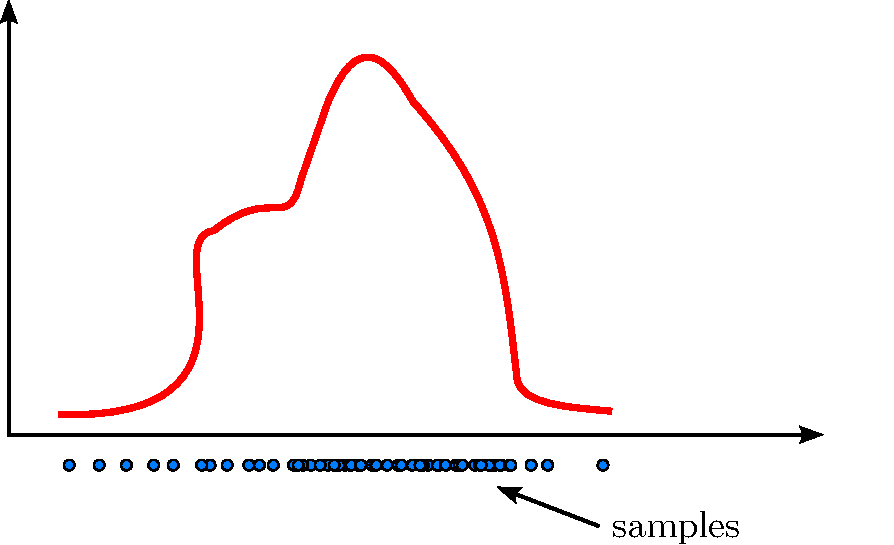
\includegraphics[width=0.5\columnwidth]{./images/particle_filter/arbitrary_distribution_samples.pdf}
    \end{center}
    
\end{frame}

\begin{frame}
    \frametitle{Utilizando Muestras con Peso}
    \note{Información extraída de Vídeo de Cyrill Stachniss https://youtu.be/MsYlueVDLI0}
    \footnotesize
    \begin{itemize}
        \item \textbf{Múltiples muestras con peso} para representar una distribución de probabilidad arbitraría
        \item Es posible reducir el número de muestras que necesitamos, si le agregamos pesos a cada muestra
        \item Mientras más peso tiene una muestra, más masa de probabilidad hay en esa región
        \item Los pesos de todas las partículas juntas deben sumar 1
        \item Al inicio, podríamos agregarle a cada muestra un peso uniforme. Por ejemplo, si tenemos $n$ muestras, entonces cada muestra tiene peso $\frac{1}{n}$
    \end{itemize}
    
    \begin{center}
        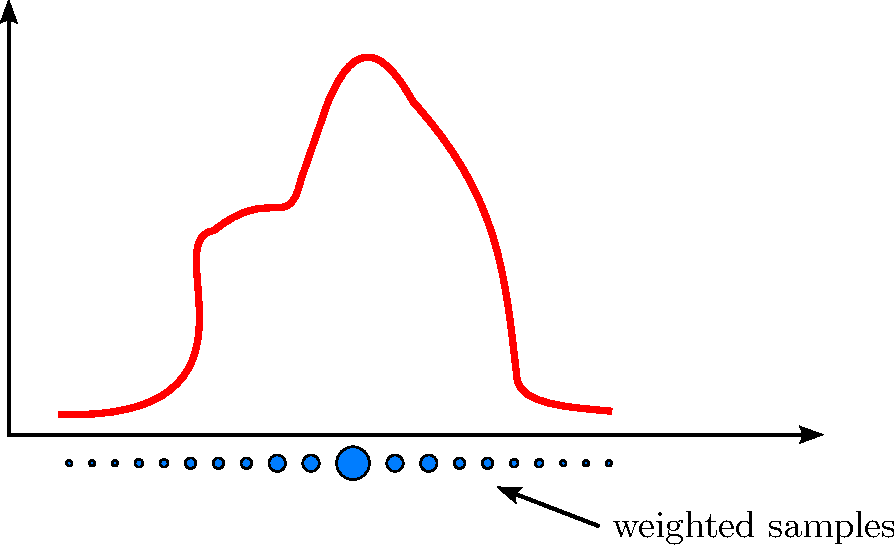
\includegraphics[width=0.5\columnwidth]{./images/particle_filter/arbitrary_distribution_weighted_samples.pdf}
    \end{center}
    
\end{frame}

\begin{frame}
    \frametitle{Filtro de Partículas (Particle Filter)}
    \note{Información extraída de Vídeo de Cyrill Stachniss https://youtu.be/MsYlueVDLI0}
    
    \footnotesize
    \begin{itemize}
        \item Notar que es una aproximación de la pdf
        \item Es importante tener un número de muestras suficientes para poder representar la fdp adecuadamente.
    \end{itemize}
    
    
\end{frame}

\begin{frame}
    \frametitle{Conjunto de Partículas}
    
    \begin{itemize}
        \item Conjunto de partículas con peso
            
        \begin{center}
            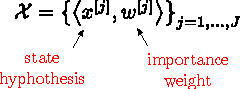
\includegraphics[width=0.5\columnwidth]{./images/particle_filter/weighted_samples.pdf}
        \end{center}

        \item Las partículas representan la posterior belief dada por
        \begin{equation*}
            p(x) = \sum_{j=1}^{J} w^{[j]} \delta_{x^{[j]}}(x)    
        \end{equation*}
        donde $\delta_{x^{[j]}}(x)$ es la función de Dirac centrada en la ubicación de la partícula $x^{[j]}$.

        \begin{equation*}
            \delta(y) = 
            \begin{cases} 
            \infty, & y = x^{[j]} \\ 
            0, & y \neq x^{[j]} 
            \end{cases};    
        \end{equation*}

        \note{La función tiende a infinito cuando $x=j$ y, para cualquier otro valor de $x$, es igual a 0.}

    \end{itemize}
   
\end{frame}


\begin{frame}
    \frametitle{Partículas para Aproximar}
    
    \begin{itemize}
        \item Partículas para aproximar una función
        
        \begin{center}
            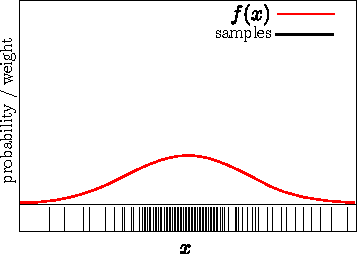
\includegraphics[width=0.45\columnwidth]{./images/particle_filter/gaussian_approximation_by_sampling.pdf}
            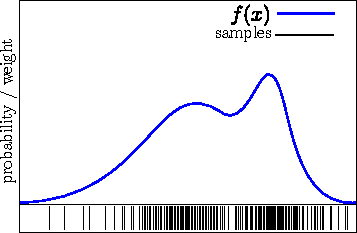
\includegraphics[width=0.45\columnwidth]{./images/particle_filter/particles_for_approximation.pdf}
        \end{center}

        \item Más partículas caen en una región, más alta es la probabilidad de la región
    \end{itemize}
    
    \begin{center}
        \alert{¿Cómo obtener dichas muestras?}
    \end{center}

\end{frame}

\begin{frame}
    \frametitle{Una Forma Cerrada de Muestreo es solo posible para Pocas Distribuciones }
    \begin{itemize}
        \item Ejemplo: Distribución Gaussiana
        
        \begin{center}
            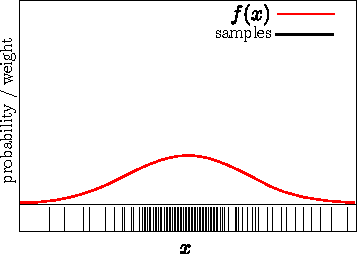
\includegraphics[width=0.5\columnwidth]{./images/particle_filter/gaussian_approximation_by_sampling.pdf}
        \end{center}
        
        \begin{equation*}
            x \leftarrow \frac{1}{2} \sum_{i=1}^{12} \text{rand}(-\sigma, \sigma)
        \end{equation*}
    \end{itemize}

    ¿Cómo samplear utilizando otra distribución?

    \note{Técnica de rejection sampling. No sé utiliza en particle filter porque es una técnica muy ineficiente.}

    \note{Técnica Importance Sampling Principle}

\end{frame}
    


\begin{frame}
    \frametitle{Principio de muestreo de importancia}
    \begin{itemize}
        \item Podemos usar una distribución diferente $\pi$ para generar muestras de $f$
        \item Considere las ``diferencias entre $\pi$ y $f$'' usando un peso $w = f(x) / \pi(x)$
        \item Target $f$
        \item Proposal $\pi$
        \item Precondición:
        $f(x) > 0 \implies \pi(x) > 0$
        \begin{center}
        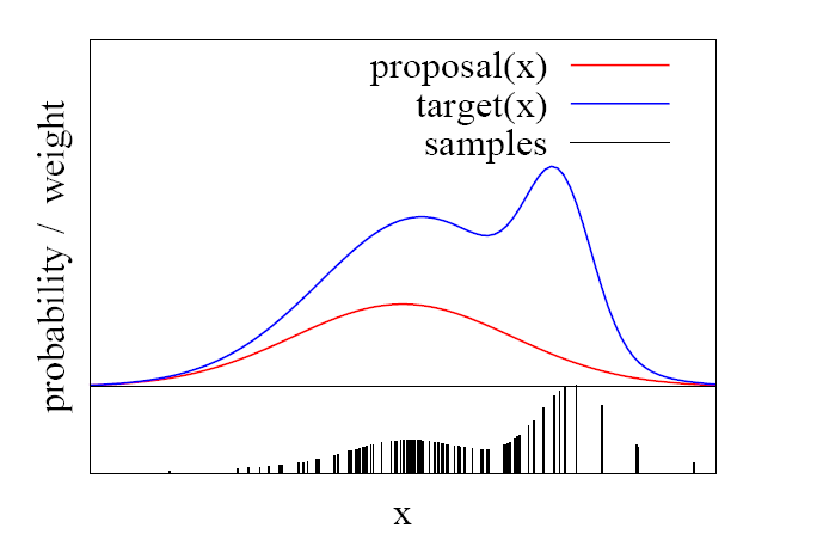
\includegraphics[width=0.45\textwidth]{./images/particle_filter/importance_sampling_principle.pdf}
        \end{center}
    \end{itemize}
\end{frame}
    
\begin{frame}
    \frametitle{Filtro de Partículas}
    \begin{itemize}
        \item Filtro Bayesiano recursivo
        \item Enfoque no paramétrico
        \item Modela la distribución mediante muestras
        \item \textbf{Predicción}: extraer de la distribución propuesta
        \item \textbf{Corrección}: ponderación por la relación entre la distribución objetivo y la propuesta
        \item \alert{¡Cuantas más muestras usemos, mejor será la estimación!}
    \end{itemize}
\end{frame}
    
\begin{frame}
    \frametitle{Algoritmo de Filtro de Partículas}
    \begin{enumerate}
        \item Muestrear las partículas utilizando la distribución propuesta.
        \begin{equation*}
            x_t^{[j]} \sim proposal(x_t | \ldots)
        \end{equation*}
        \item Calcular los pesos de importancia
        \begin{equation*}
            w_t^{[j]} = \frac{target(x_t^{[j]})}{proposal(x_t^{[j]})}
        \end{equation*}
        \item Resampling: Tomar la partícula $i$ con probabilidad $w_t^{[j]}$ y repetir $J$ veces 
    \end{enumerate}
    \note{Reemplazar muestras improbables por otras más probables}
\end{frame}

\begin{frame}
    \frametitle{Algoritmo de Filtro de Partículas}
    \begin{algorithmic}[1]
    \Procedure{ParticleFilter}{$\mathcal{X}_{t-1}, u_{t}, z_{t}$}:
    \State $\bar{\mathcal{X}}_t = \mathcal{X}_t = \emptyset$
    \For{$j = 1$ to $J$}
        \State sample $x_t^{[j]} \sim \pi(x_t)$
        \State $w_t^{[j]} = \dfrac{p(x_t^{[j]})}{\pi(x_{t}^{[j]})}$
        \State $\bar{\mathcal{X}}_t = \bar{\mathcal{X}}_t + \langle x_t^{[j]}, w_t^{[j]}\rangle$
    \EndFor
    \For{$j = 1$ to $M$}
        \State Draw $i$ with probability $\propto w_t^{[i]}$
        \State Add $x_t^{[i]}$ to $\mathcal{X}_t$
    \EndFor
    \State return $\mathcal{X}_t$
    \EndProcedure
    \end{algorithmic}
\end{frame}


\begin{frame}
    \frametitle{Monte Carlo Localization}

    Monte Carlo Localization: Filtro de Partículas para la localización de un robot

\end{frame}


% \begin{frame}
%     \frametitle{Monte Carlo Localization}

%     \begin{center}
%         \includegraphics[width=0.37\textwidth]{./images/particle_filter/monte_carlo_localization_example.pdf}
%     \end{center}

% \end{frame}

\begin{frame}
    \frametitle{Monte Carlo Localization}
    \begin{itemize}
        \item Cada partícula es una hipótesis de la pose
        \item Proposal es el motion model
        \begin{equation*}
            x_t^{[j]} \sim p(x_t \, | \, x_{t-1}, u_t)
        \end{equation*}
        \item Corrección vía el observation model
        \begin{equation*}
            w_t^{[j]} = \frac{target}{proposal} \propto p(z_t \, | \, x_t, m)
        \end{equation*}
    \end{itemize}
\end{frame}

    
\begin{frame}
    \frametitle{Filtro de Partículas para Localización}
    \begin{algorithmic}[1]
        \Procedure{ParticleFilter}{$\mathcal{X}_{t-1}, u_{t}, z_{t}$}
        \State $\bar{\mathcal{X}}_t = \mathcal{X}_t = \emptyset$
        \For{$j = 1$ to $J$}
            \State Sample $x_t^{[j]} \sim p(x_t \, | \, u_t, x_{t-1}^{[j]})$
            \State $w_t^{[j]} = p(z_t \, | \, x_t^{[j]})$
            \State $\bar{\mathcal{X}}_t = \bar{\mathcal{X}}_t + \langle x_t^{[j]}, w_t^{[j]}\rangle$
        \EndFor
        \For{$i = 1$ to $J$}
            \State Draw $i \in 1,\ldots,J$ with probability $\propto w_t^{[i]}$
            \State Add $x_t^{[i]}$ to $\mathcal{X}_t$
        \EndFor
        \State return $\mathcal{X}_t$
    \EndProcedure
    \end{algorithmic}
\end{frame}
    
\begin{frame}
    \frametitle{Monte Carlo Localization - Paso de Corrección}

    \begin{center}
        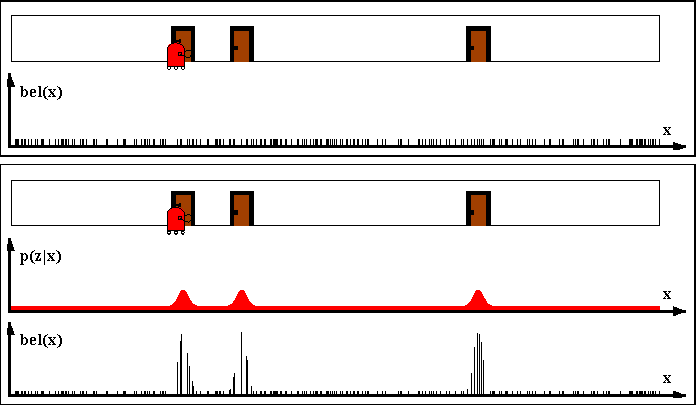
\includegraphics[width=0.8\textwidth]{./images/particle_filter/monte_carlo_correction.pdf}
    \end{center}

\end{frame}

\begin{frame}
    \frametitle{Monte Carlo Localization - Remuestreo y Predicción}

    \begin{center}
        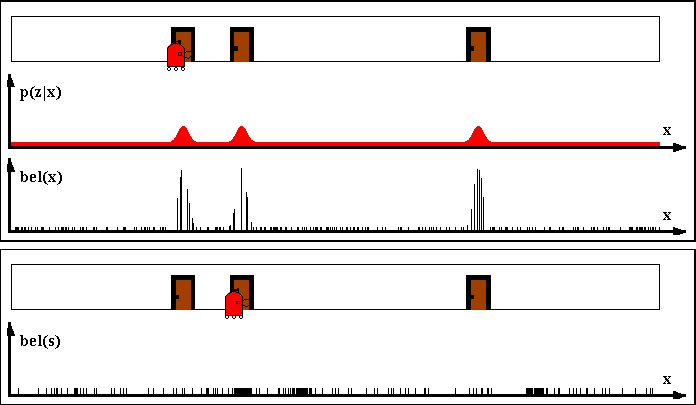
\includegraphics[width=0.8\textwidth]{./images/particle_filter/monte_carlo_resample_and_predict.pdf}
    \end{center}

\end{frame}

\begin{frame}
    \frametitle{Monte Carlo Localization - Paso de Corrección 2}

    \begin{center}
        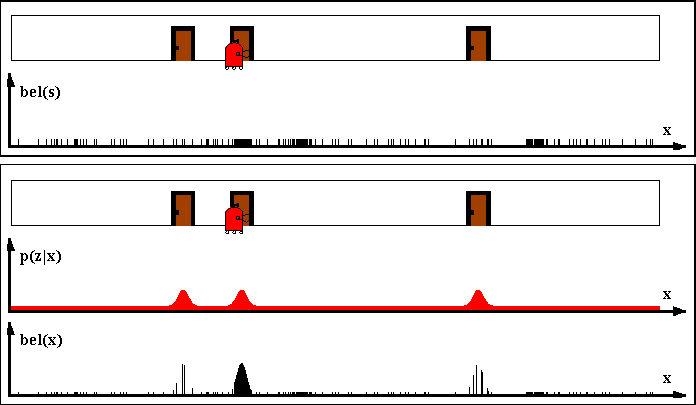
\includegraphics[width=0.8\textwidth]{./images/particle_filter/monte_carlo_correction2.pdf}
    \end{center}

\end{frame}

\begin{frame}
    \frametitle{Monte Carlo Localization - Remuestreo y Predicción 2}

    \begin{center}
        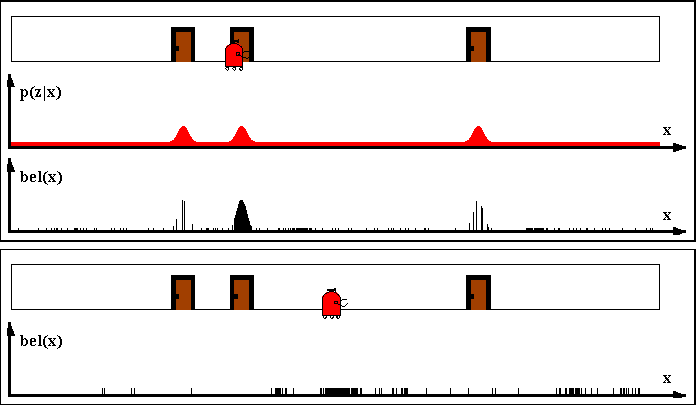
\includegraphics[width=0.8\textwidth]{./images/particle_filter/monte_carlo_resample_and_predict2.pdf}
    \end{center}

\end{frame}


\begin{frame}
    \frametitle{Resampling}
    \begin{itemize}
        \item Tomar la partícula $i$ con probabilidad $w_t^{[i]}$. Repetir $J$ veces.
        \item Informalmente: ``Reemplazar muestras improbables por otras más probables''
        \item Supervivencia del más apto
        \item ``Truco'' para evitar que muchas muestras cubran estados improbables
        \item Necesario, ya que tenemos un número limitado de muestras
    \end{itemize}
\end{frame}
    
\begin{frame}
    \frametitle{Métodos de Resampling}
    \centering
    \only<1>{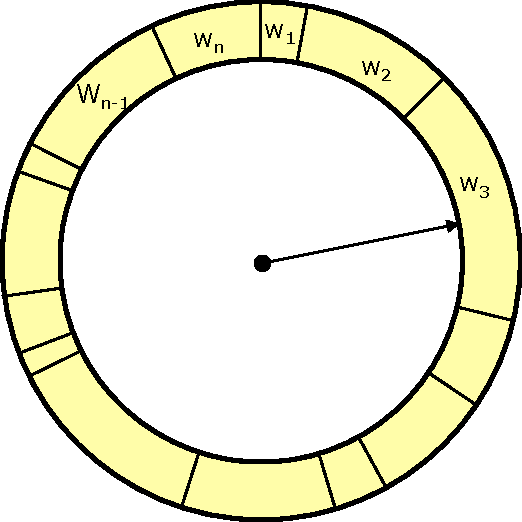
\includegraphics[width=0.4\textwidth]{./images/particle_filter/resampling_rulette_wheel1.pdf}}
    \only<2>{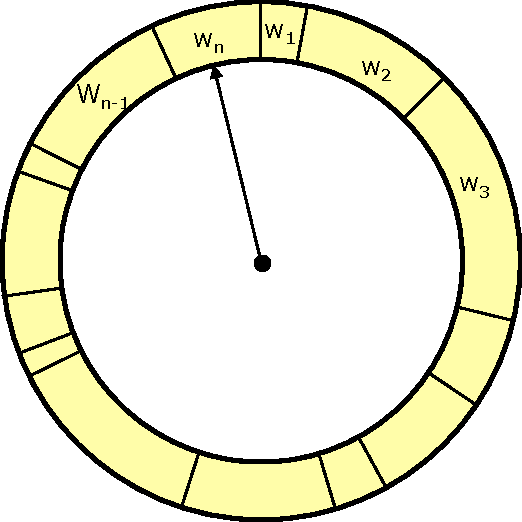
\includegraphics[width=0.4\textwidth]{./images/particle_filter/resampling_rulette_wheel2.pdf}}
    \only<3>{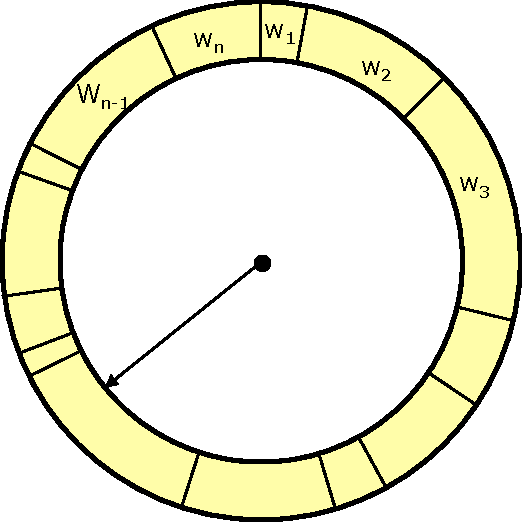
\includegraphics[width=0.4\textwidth]{./images/particle_filter/resampling_rulette_wheel3.pdf}}

    \only<3>{
        \begin{itemize}
            \item Ruleta
            \item Búsqueda binaria para saber en qué bucket cae la bola ($O(J \log(J))$)
        \end{itemize}
        \note{Los buckets de la ruleta representan los pesos de las partículas. Mientras más grande el bucket, más probable es que esta partícula sea seleccionada.}
        \note{Tenemos que hacerlo J veces. Tenemos que encontrar dónde cae la bola. Esto lo podemos hacer con binary-search. La suma de todos los pesos de la ruleta es 1. Si tiramos un número random entre 0 y 1 entonces con búsqueda binaria podemos saber en qué bucket cae.}
    }
\end{frame}

\begin{frame}
    \frametitle{Métodos de Resampling}
    \centering
    \only<1>{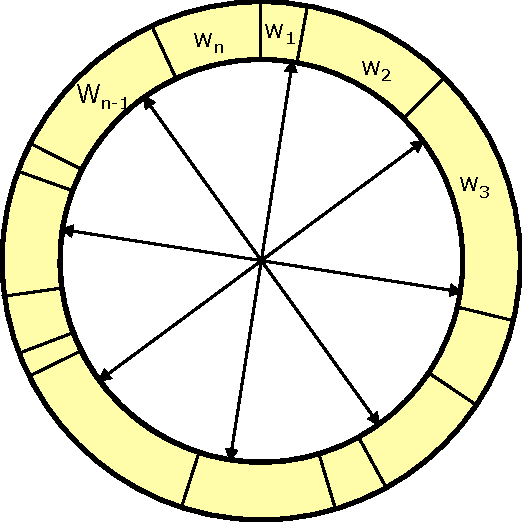
\includegraphics[width=0.4\textwidth]{./images/particle_filter/resampling_stochastic_universal_sampling1.pdf}}
    \only<2>{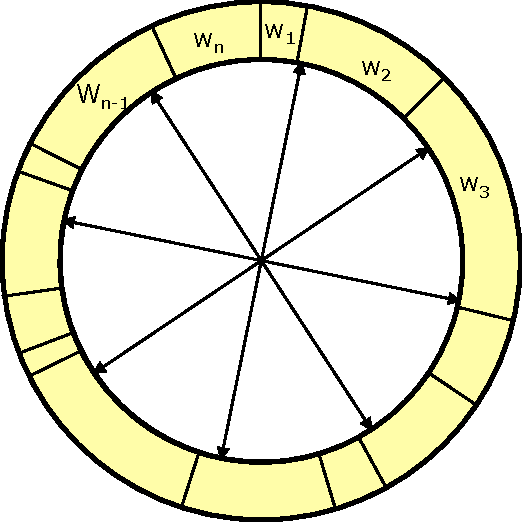
\includegraphics[width=0.4\textwidth]{./images/particle_filter/resampling_stochastic_universal_sampling2.pdf}}
    
    \only<2>{
    \begin{itemize}
        \item Stochastic universal sampling (utilizando $n$ flechas)
        \item Baja varianza
        \item $O(J)$
    \end{itemize}
    \note{Utilizando on flechas y poniendolas equidistantes. Rotamos todas juntas y elejimos de a n partículas. Por tanto cuando, tiro un número random ahora se seleccionan n partículas.}
    \note{Ejemplo 8 flechas distante 45 grados una de otra.}
    }
\end{frame}
    
\begin{frame}
    \frametitle{Low Variance Resampling}
    \begin{algorithmic}[1]
    \State $\bar{\mathcal{X}}_t = \emptyset$
    \State $r = \text{rand}(0; M^{-1})$
    \State $c = w_t^{[1]}$
    \State $i = 1$
    \For{$m = 1$ to $M$}
        \State $U = r + (m - 1) \cdot M^{-1}$
        \While{$U > c$}
            \State $i = i + 1$
            \State $c = c + w_t^{[i]}$
        \EndWhile
        \State Add $x_t^{[i]}$ to $\bar{\mathcal{X}}_t$
    \EndFor
    \State Return $\bar{\mathcal{X}}_t$
    \end{algorithmic}
\end{frame}

\begin{frame}
    \frametitle{Desventajas}
    \begin{itemize}
        \item No escala bien para espacios de alta dimensionalidad
        \item Problemático en situaciones con mucha incertidumbre
        \item Problema agotamiento de partículas
    \end{itemize}
\end{frame}

\begin{frame}
    \frametitle{Ventajas}
    \begin{itemize}
        \item Puede trabajar con distribuciones no Gaussianas
        \item Funciona bien en espacios de baja dimensionalidad
        \item Puede manejar ambiguedades en la asociación de los datos
        \item Puede incorporar fácilmente diferentes modalidades de sensado
        \item Robusto
        \item Fácil de implementar
    \end{itemize}
\end{frame}

\begin{frame}
    \frametitle{Resumen – Particle Filter}
    \begin{itemize}
        \item Los filtros de partículas son filtros bayesianos recursivos y no paramétricos
        \item El Posterior Belief se representa mediante un conjunto de muestras ponderadas
        \item No se limita a Gaussianas
        \item Proposal para extraer muestras en $t+1$
        \item Peso para tener en cuenta las diferencias entre la proposal y el target
    \end{itemize}
\end{frame}
    
\begin{frame}
    \frametitle{Resumen – Localización con PF}
    \begin{itemize}
        \item Las partículas se propagan según el modelo de movimiento
        \item Se ponderan según la probabilidad de la observación
        \item Se denomina Localización de Monte Carlo (MCL)
        \item La MCL es un gold standard para la localización de robots móviles en entornos \emph{indoor}
    \end{itemize}
\end{frame}



\begin{frame}
    \frametitle{Material para Particle Filter}
    
    \begin{itemize}
        \item Información extraída de Vídeo de Cyrill Stachniss https://youtu.be/MsYlueVDLI0
        \item https://rse-lab.cs.washington.edu/projects/mcl/
        \item http://ais.informatik.uni-freiburg.de/teaching/ws12/mapping/pdf/slam09-particle-filter.pdf
    \end{itemize}
   
\end{frame}


\begin{frame}
    \frametitle{TODO}
    \note{Información extraída de Vídeo de Cyrill Stachniss https://youtu.be/MsYlueVDLI0}
    \note{https://rse-lab.cs.washington.edu/projects/mcl/}
    
    \TODO{UTILIZAR LAS SLIDES DEL SEMINARIO}
    
    
\end{frame}


    
